\newpage
\section{CÁC PHÉP TOÁN TRÊN TẬP HỢP}
\subsection{LÝ THUYẾT CẦN NHỚ}
\subsubsection{Hợp và giao của các tập hợp}
\iconMT\indam{Định nghĩa:}
\begin{boxdn}
		Cho hai tập hợp $A$ và $B$.
	\begin{itemize}
		\item Tập hợp các phần tử thuộc $A$ hoặc thuộc $B$ gọi là \textbf{hợp} của hai tập hợp $A$ và $B$, kí hiệu $A \cup B$.\immini{		
		\begin{itemize}
			\item $A \cup B = \{x \mid x \in A \text{ hoặc } x \in B\}$.
			\item $x \in A \cup B \Leftrightarrow 
			\begin{cases}
				x \in A \\
				x \in B.
			\end{cases}$
		\end{itemize}}
	{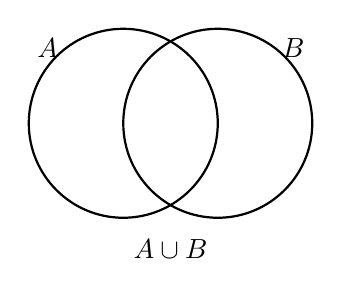
\begin{tikzpicture}[scale=.8]
			\draw[thick] (0,0) circle(1.5cm);
			\draw[thick] (1.5,0) circle(1.5cm);
			\node at (-1.2,1.2) {$A$};
			\node at (2.7,1.2) {$B$};
			\node at (0.75,-2) {$A \cup B$};
			%					\node at (0.75,-2.3) {a)};
		\end{tikzpicture}}
		\item Tập hợp các phần tử thuộc cả hai tập hợp $A$ và $B$ gọi là \textbf{giao} của hai tập hợp $A$ và $B$, kí hiệu $A \cap B$.
		\immini{\begin{itemize}
			\item $A \cap B = \{x \mid x \in A \text{ và } x \in B\}$.
			\item $x \in A \cap B \Leftrightarrow 
			\begin{cases}
				x \in A \\
				x \in B.
			\end{cases}$
		\end{itemize}}
	{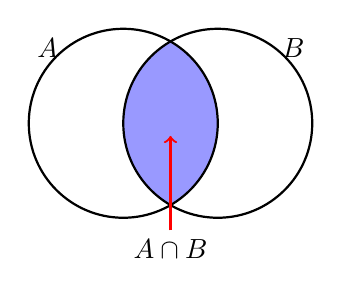
\begin{tikzpicture}[scale=.8]
			% Tô màu vùng giao
			\begin{scope}
				\clip (0,0) circle(1.5cm);
				\fill[blue!40] (1.5,0) circle(1.5cm);
			\end{scope}
			
			% Hai tập A và B
			\draw[thick] (0,0) circle(1.5cm);
			\draw[thick] (1.5,0) circle(1.5cm);
			
			\node at (-1.2,1.2) {$A$};
			\node at (2.7,1.2) {$B$};
			
			% Mũi tên từ nhãn đến vùng giao
			\draw[red,->,thick] (0.75,-1.7) -- (0.75,-0.2);
			
			\node at (0.75,-2) {$A \cap B$};
%			\node at (0.75,-2.3) {b)};
	\end{tikzpicture}}
	\end{itemize}
\end{boxdn}
\begin{nx}
	\begin{itemize}
		\item Nếu $A$ và $B$ là hai tập hợp hữu hạn thì $n(A\cup B)=n(A)+n(B)-n(A\cap B)$.
		\item Đặt biệt nếu $A$ và $B$ không có phần tử chung, tức $A\cap B=\varnothing$ thì $n(A\cup B)=n(A)+n(B)$.
	\end{itemize}
\end{nx}
\subsection{Hiệu của hai tập hợp, phần bù của tập con}
\immini{Cho hai tập hợp $A$ và $B$.\\
Tập hợp các phần tử thuộc $A$ nhưng không thuộc $B$ gọi là \textbf{hiệu} của $A$ và $B$, kí hiệu $A \setminus B$.
\[
A \setminus B = \{x \mid x \in A \text{ và } x \notin B\}.
\]
\[
x \in A \setminus B \Leftrightarrow \heva{&x\in A\\& x\notin B.}
\]
Nếu $A \subset U$ thì hiệu $U \setminus A$ được gọi là \textit{phần bù} của $A$ trong $U$, kí hiệu $\mathrm{C}_UA$.
}
{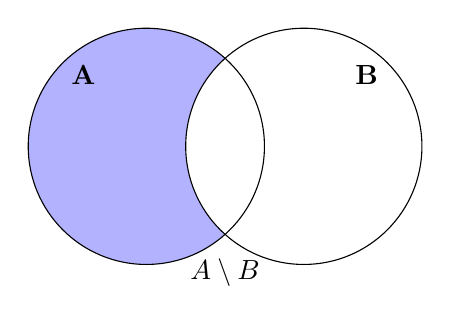
\begin{tikzpicture}
		
		% Tô màu phần A \ B
		\begin{scope}
			\clip (-1,0) circle (1.5);         % Vùng của A
			\fill[blue!30] (-1,0) circle (1.5); % Tô toàn bộ A
			\fill[white] (1,0) circle (1.5);    % Trừ đi phần giao với B
		\end{scope}
		
		% Vẽ đường viền hai tập A và B
		\draw (-1,0) circle (1.5); % Tập A
		\draw (1,0) circle (1.5);  % Tập B
		
		% Nhãn các tập
		\node at (-1.8,0.9) {\textbf{A}};
		\node at (1.8,0.9) {\textbf{B}};
		\node at (0,-1.6) {\textbf{$A \setminus B$}};
		
\end{tikzpicture}\\
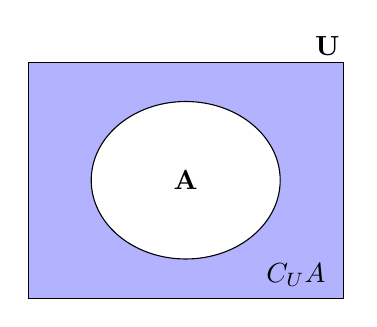
\begin{tikzpicture}
	
	% Tô màu phần bù của A
	\fill[blue!30] (-2,-1.5) rectangle (2,1.5); % Toàn bộ U tô màu
	
	\begin{scope}
		\clip (-2,-1.5) rectangle (2,1.5); % Giới hạn tô trong U
		\fill[white] (0,0) ellipse (1.2 and 1); % Loại bỏ vùng A
	\end{scope}
	
	% Vẽ biên giới của U và A
	\draw (-2,-1.5) rectangle (2,1.5); % U
	\draw (0,0) ellipse (1.2 and 1);   % A
	
	% Gán nhãn
	\node at (0,0) {\textbf{A}};
	\node at (1.4,-1.2) {\textbf{$C_U A$}};
	\node at (1.8,1.7) {\textbf{U}};
	
\end{tikzpicture}

}
\begin{note}
	Trong các chương sau, để tìm các tập hợp là giao, hợp, hiệu, phần bù của những tập con của tập số thực, ta thường vẽ sơ đồ trên trục số.
\end{note}

\subsection{PHÂN LOẠI VÀ PHƯƠNG PHÁP GIẢI TOÁN}
\begin{dang}{Giao, hợp của hai tập hợp rời rạc}
\textbf{Phương pháp giải:}
\begin{itemize}
	\item \textbf{Tìm giao hai tập hợp $A$ và $B$:}
	\begin{itemize}
		\item So sánh từng phần tử của tập $A$ với các phần tử của tập $B$.
		\item Ghi lại các phần tử có mặt trong cả hai tập.
	\end{itemize}
	
	\item \textbf{Tìm hợp hai tập hợp $A$ và $B$:}
	\begin{itemize}
		\item Gộp tất cả phần tử của $A$ và $B$ lại thành một tập.
		\item Loại bỏ các phần tử trùng nhau.
	\end{itemize}
\end{itemize}	
\end{dang}
%%%=============VD_1=============%%%
\begin{vd}%[0D1N3-1]
	Cho hai tập hợp $A = \{1; 2; 3; 4\}$ và $B = \{3; 4; 5; 6\}$. Tìm $A \cup B$ và $A \cap B$.
	\loigiai
	{
		Ta có
		\begin{multicols}{2}
			\begin{itemize}
				\item $A \cup B = \{1; 2; 3; 4; 5; 6\}$.
				\item $A \cap B = \{3; 4\}$.
			\end{itemize}
		\end{multicols}
	}
\end{vd}
%%%=============================%%%

%%%=============VD_2=============%%%
\begin{vd}%[0D1H3-1]
	Cho hai tập hợp $A = \{x \in \mathbb{N} \mid x < 6\}$ và $B = \{x \in \mathbb{N} \mid x \text{ chẵn và } x \leq 10\}$. Tìm $A \cap B$ và $A \cup B$.
	\loigiai
	{
		Ta có
		\begin{multicols}{2}
			\begin{itemize}
				\item $A = \{0; 1; 2; 3; 4; 5\}$.
				\item $A \cap B = \{0; 2; 4\}$.
				\item $B = \{0; 2; 4; 6; 8; 10\}$.
				\item $A \cup B = \{0; 1; 2; 3; 4; 5; 6; 8; 10\}$.
			\end{itemize}
		\end{multicols}
	}
\end{vd}
%%%=============================%%%

%%%=============VD_3=============%%%
\begin{vd}%[0D1H3-1]%[0D1H3-3]
	\begin{enumerate}
		\item Cho tập hợp $A=\{a,b,c,1,2,3\}$, $B=\{a,b,2,3,4,5\}$. Xác định tập hợp $A\cup B$.
		\item Biết $D=\{(x;y)|x,y\in \mathbb{R},2x-y=1\}$, $E=\{(x;y)|x,y\in \mathbb{R},x+y=5\}$. Tìm $D\cap E$.
	\end{enumerate}
	\loigiai{
		\begin{enumerate}
			\item Ta có $A\cup B=\{a,b,c,1,2,3,4,5\}$.
			\item Ta có $(x;y)\in D\cap E \Leftrightarrow \heva{&2x-y=1\\&x+y=5}\Leftrightarrow \heva{&x=2\\&y=3.}$\\
			Vậy $D\cap E=\{(2;3)\}$.
		\end{enumerate}
	}
\end{vd}
%%%=============================%%%

\begin{dang}{Hiệu và phần bù của hai tập hợp rời rạc}
	\textbf{Phương pháp giải:}
\begin{itemize}
	\item \textbf{Tìm hiệu hai tập hợp $A$ và $B$ ($A \setminus B$):}
	\begin{itemize}
		\item Lấy các phần tử thuộc $A$ nhưng không thuộc $B$.
		\item Ký hiệu: $A \setminus B = \{x \mid x \in A \text{ và } x \notin B\}$.
	\end{itemize}
	
	\item \textbf{Tìm phần bù của tập $A$ trong $U$ (vũ trụ):}
	\begin{itemize}
		\item Lấy các phần tử thuộc tập vũ trụ $U$ nhưng không thuộc $A$.
		\item Ký hiệu: $A' = U \setminus A = \{x \in U \mid x \notin A\}$.
	\end{itemize}
\end{itemize}
\end{dang}
\setcounter{vd}{0}
%%%=============VD_1=============%%%
\begin{vd}%[0D1N3-2]
	Cho hai tập hợp $A = \{1; 2; 3; 4; 5\}$ và $B = \{3; 4; 6; 7\}$. Tìm hiệu các tập $A \setminus B$ và $B \setminus A$.
	\loigiai
	{
		Ta có
		\begin{multicols}{2}
			\begin{itemize}
				\item $A \setminus B = \{1; 2; 5\}$.
				\item $B \setminus A = \{6; 7\}$.
			\end{itemize}
		\end{multicols}
	}
\end{vd}
%%%=============================%%%

%%%=============VD_2=============%%%
\begin{vd}%[0D1N3-2]
	Cho tập $U = \{0; 1; 2; 3; 4; 5; 6\}$ và hai tập con $A = \{1; 3; 5\}$, $B = \{2; 3; 4; 6\}$. Tìm phần bù của $A$ và $B$ trong $U$.
	\loigiai
	{
		Ta có
		\begin{multicols}{2}
			\begin{itemize}
				\item $\mathrm{C}_U A = U \setminus A = \{0; 2; 4; 6\}$.
				\item $\mathrm{C}_U B = U \setminus B = \{0; 1; 5\}$.
			\end{itemize}
		\end{multicols}
	}
\end{vd}
%%%=============================%%%

%%%=============VD_3=============%%%
\begin{vd}%[0D1H3-2]
	\begin{enumerate}
		\item Liệt kê các phần tử của tập hợp: $M=\left\{x \in \mathbb{Z}|(2x-6) \cdot\left(2x^2-7x-9\right)=0\right\}$.
		\item Cho hai tập hợp $A=\{0; 1; 2; 3\}$ và $B=\{1; 3; 5; 7; 9\}$. Tìm $A\cap B$ và $A\setminus B$.
	\end{enumerate}
	\loigiai{
		\begin{enumerate}
			\item Ta có $(2x-6) \cdot\left(2x^2-7x-9\right)=0\Leftrightarrow \hoac{&x=3\\&x=-1\\&x=\dfrac{9}{2} \text{ (loại).}}$\\
			Vậy $M=\{-1;3\}$.
			\item $A\cap B=\{1;3\}$ và $A\setminus B=\{0;2\}$.
		\end{enumerate}
	}
\end{vd}
%%%=============================%%%
\begin{dang}{Giao và hợp dùng đoạn, khoảng}
	\textbf{Phương pháp giải:} Cho $A$, $B$ là hai tập con của tập số thực.
	\begin{itemize}
		\item Để tìm $A \cap B$, ta làm như sau:
		\begin{itemize}
			\item Biểu diễn $A$, $B$ trên trục số; gạch bỏ phần không thuộc $A$, $B$.
			\item Phần không bị gạch là $A \cap B$.
		\end{itemize}
		\item Để tìm $A \cup B$, ta làm như sau:
		\begin{itemize}
			\item Biểu diễn $A$, $B$ trên trục số; tô đậm phần thuộc $A$, $B$.
			\item Phần tô đậm là $A \cup B$.
		\end{itemize}
	\end{itemize}
\end{dang}
\setcounter{vd}{0}
%%%=============VD_1=============%%%
\begin{vd}%[0D1N3-3]
	Cho hai tập
	\[ A = (-5;2), \quad B = (-\infty;0] \]
	Hãy xác định: tập hợp $A \cup B$.
	\loigiai{
		Tập $A$ gồm các phần tử lớn hơn $-5$ và nhỏ hơn $2$. Tập $B$ gồm các phần tử nhỏ hơn hoặc bằng $0$.
		\[ A \cup B = (-\infty;2). \]
		\begin{center}
			\begin{tikzpicture}[scale=1, font=\footnotesize, line join=round, line cap=round,>=stealth]
				\def\xmin{-8}; \def\xmax{4};
				% A = (-5;2)
				\draw[->] (\xmin,0)--(\xmax,0);
				\node (a0) at (-5,0){(};
				\node (b0) at (2,0){)};
				\draw (a0.-90)node[below]{$-5$} (b0.-90)node[below]{$2$};
				\draw[draw=none, pattern=north west lines] (\xmin,0.1)--($(a0)+(90:0.1)$)--($(a0)+(-90:0.1)$)--(\xmin,-0.1)--cycle;
				\draw[draw=none, pattern=north west lines] ($(b0)+(90:0.1)$)--(\xmax,0.1)--(\xmax,-0.1)--($(b0)+(-90:0.1)$)--cycle;
				
				% B = (-inf;0]
				\draw[->] (\xmin,-1)--(\xmax,-1);
				\node (b1) at (0,-1){]};
				\draw (b1.-90)node[below]{$0$};
				\draw[draw=none, pattern=north west lines] ($(b1)+(90:0.1)$)--(\xmax,-0.9)--(\xmax,-1.1)--($(b1)+(-90:0.1)$)--cycle;
			\end{tikzpicture}
		\end{center}
	}
\end{vd}
%%%=============================%%%

%%%=============VD_2=============%%%
\begin{vd}%[0D1N3-3]
	Cho hai tập hợp $A = (2; 6)$ và $B = [4; 8)$.
	\begin{enumerate}
		\item Dùng biểu diễn hình học để minh họa $A$, $B$, $A \cap B$, $A \cup B$.
		\item Xác định $A \cap B$ và $A \cup B$.
	\end{enumerate}
	\loigiai{
		\begin{enumerate}
			\item Biểu diễn trên trục số:
			
			\begin{center}
				\begin{tikzpicture}
					\draw[->] (0,0) -- (9,0) node[right] {$x$};
					
					% A
					\draw[thick] (2,0.5) -- (6,0.5);
					\draw[fill=white] (2,0.5) circle (2pt) node[below] {$2$};
					\draw[fill=white] (6,0.5) circle (2pt) node[below] {$6$};
					\node at (1.2,0.5) {$A:$};
					
					% B
					\draw[thick] (4,1) -- (8,1);
					\filldraw (4,1) circle (2pt) node[above] {$4$};
					\draw[fill=white] (8,1) circle (2pt) node[above] {$8$};
					\node at (1.2,1) {$B:$};
					
					% Giao A ∩ B
					\draw[pattern=north east lines, pattern color=blue] (4,1.5) rectangle (6,1.8);
					\filldraw (4,1.65) circle (2pt);
					\draw[fill=white] (6,1.65) circle (2pt);
					\draw (4,1.65) -- (6,1.65);
					\node at (1.2,1.65) {$A \cap B:$};
					
					% Hợp A ∪ B
					\draw[pattern=north west lines, pattern color=red] (2,2.2) rectangle (8,2.5);
					\draw[fill=white] (2,2.35) circle (2pt);
					\draw[fill=white] (8,2.35) circle (2pt);
					\draw (2,2.35) -- (8,2.35);
					\node at (1.2,2.35) {$A \cup B:$};
				\end{tikzpicture}
			\end{center}
			\item Ta có
			\[
			A \cap B = [4;6),\quad A \cup B = (2;8).
			\]
		\end{enumerate}
	}
\end{vd}
%%%=============================%%%

%%%=============VD_3=============%%%
\begin{vd}%[0D1H3-3]
	Cho hai tập hợp $A = [-3; 1]$ và $B = (0; 4]$.
	\begin{enumerate}
		\item Biểu diễn các tập hợp $A$, $B$, $A \cap B$, $A \cup B$, $C$ trên trục số.
		\item Tìm $A \cap B$ và $A \cup B$.
		\item Tập hợp $C = A \setminus B$. Hãy xác định $C$.
	\end{enumerate}
	\loigiai{
		\begin{enumerate}
			\item Biểu diễn:
			
			\begin{center}
				\begin{tikzpicture}
					\draw[->] (0,0) -- (10,0) node[right] {$x$};
					
					% A
					\draw[thick] (2,0.5) -- (6.8,0.5);
					\filldraw (2,0.5) circle (2pt) node[below] {$-3$};
					\filldraw (6.8,0.5) circle (2pt) node[below] {$1$};
					\node at (1,0.5) {$A:$};
					
					% B
					\draw[thick] (6,1) -- (9,1);
					\draw[fill=white] (6,1) circle (2pt) node[above] {$0$};
					\filldraw (9,1) circle (2pt) node[above] {$4$};
					\node at (1,1) {$B:$};
					
					% Giao A ∩ B
					\draw[pattern=north east lines, pattern color=blue] (6,1.5) rectangle (6.8,1.8);
					\draw[fill=white] (6,1.65) circle (2pt);
					\filldraw (6.8,1.65) circle (2pt);
					\draw (6,1.65) -- (6.8,1.65);
					\node at (1,1.65) {$A \cap B:$};
					
					% Hợp A ∪ B
					\draw[pattern=north west lines, pattern color=red] (2,2.2) rectangle (9,2.5);
					\filldraw (2,2.35) circle (2pt);
					\filldraw (9,2.35) circle (2pt);
					\draw (2,2.35) -- (9,2.35);
					\node at (1,2.35) {$A \cup B:$};
					
					% C = A \ B
					\draw[pattern=crosshatch dots, pattern color=gray] (2,2.9) rectangle (6,3.2);
					\filldraw (2,3.05) circle (2pt);
					\draw[fill=white] (6,3.05) circle (2pt);
					\draw (2,3.05) -- (6,3.05);
					\filldraw (6,3.05) circle (2pt); % điểm 1 riêng biệt
					\node at (1,3.05) {$A \setminus B:$};
				\end{tikzpicture}
			\end{center}
			\item Ta có
			\[
			A \cap B = (0;1],\quad A \cup B = [-3;4].
			\]
			\item Tập $C = A \setminus B = [-3;0]$.
		\end{enumerate}
	}
\end{vd}
%%%=============================%%%

\begin{dang}{Hiệu và phần bù dùng đoạn, khoảng}
	\textbf{Phương pháp:} Cho $A$, $B$ là hai tập con của tập số thực. Để tìm $A \setminus B$, ta làm như sau:
\begin{itemize}
	\item Biểu diễn $A$, $B$ trên trục số; tô đậm phần thuộc $A$, gạch bỏ phần thuộc $B$.
	\item Phần tô đậm mà không bị gạch là $A \setminus B$.
\end{itemize}
Dựa vào các bước biểu diễn trên trục số để xác định các tập giao, hợp, hiệu theo thứ tự.
\end{dang}
\setcounter{vd}{0}
%%%=============VD_1=============%%%
\begin{vd}%[0D1N3-4]
	Cho hai tập:
	\[ A = [0;5], \quad B = (3;+\infty).\]
	Hãy xác định: tập hợp $A \setminus B$.
	\loigiai{Biển diễn $A$, $B$ trên trục số
		\begin{center}
			\begin{tikzpicture}[scale=1, font=\footnotesize, line join=round, line cap=round,>=stealth]
				\def\xmin{-2}; \def\xmax{10};
				% A = [0;5]
				\draw[->] (\xmin,0)--(\xmax,0);
				\node (a0) at (0,0){[};
				\node (b0) at (5,0){]};
				\draw (a0.-90)node[below]{$0$} (b0.-90)node[below]{$5$};
				\draw[draw=none, pattern=north west lines] ($(b0)+(90:0.1)$)--(\xmax,0.1)--(\xmax,-0.1)--($(b0)+(-90:0.1)$)--cycle;
				\draw[draw=none, pattern=north west lines] ($(a0)+(90:0.1)$)--(\xmin,0.1)--(\xmin,-0.1)--($(a0)+(-90:0.1)$)--cycle;
				
				% B = (3;+inf)
				\draw[->] (\xmin,-1)--(\xmax,-1);
				\node (a1) at (3,-1){(};
				\draw (a1.-90)node[below]{$3$};
				\draw[draw=none, pattern=north west lines] (\xmin,-0.9)--($(a1)+(90:0.1)$)--($(a1)+(-90:0.1)$)--(\xmin,-1.1)--cycle;
			\end{tikzpicture}
		\end{center}
		Từ biểu diễn trên suy ra $A \setminus B = [0;3]$.
	}
\end{vd}
%%%=============================%%%

%%%=============VD_2=============%%%
\begin{vd}%[0D1N3-4]
	Cho hai tập:
	\[ A = [-4;3), \quad B = (-2;5].\]
	Hãy xác định: Tập hợp $A \setminus B$.
	\loigiai{
		Biểu diễn $A$, $B$ trên trục số
		\begin{center}
			\begin{tikzpicture}[scale=1, font=\footnotesize, line join=round, line cap=round,>=stealth]
				\def\xmin{-6}; \def\xmax{6};
				% A = [-4;3)
				\draw[->] (\xmin,0)--(\xmax,0);
				\node (a0) at (-4,0){[};
				\node (b0) at (3,0){)};
				\draw (a0.-90)node[below]{$-4$} (b0.-90)node[below]{$3$};
				\draw[draw=none, pattern=north west lines] (-2,0.1)--(\xmax,0.1)--(\xmax,-0.1)--(-2,-0.1)--cycle;
				
				% B = (-2;5]
				\draw[->] (\xmin,-1)--(\xmax,-1);
				\node (a1) at (-2,-1){(};
				\node (b1) at (5,-1){]};
				\draw (a1.-90)node[below]{$-2$} (b1.-90)node[below]{$5$};
				\draw[draw=none, pattern=north west lines] (\xmin,-0.9)--(-2,-0.9)--(-2,-1.1)--(\xmin,-1.1)--cycle;
				\draw[draw=none, pattern=north west lines] (\xmax,-0.9)--(5,-0.9)--(5,-1.1)--(\xmax,-1.1)--cycle;
			\end{tikzpicture}
		\end{center}
		Từ biểu diễn trên suy ra $A \setminus B = [-4;-2]$.
	}
\end{vd}
%%%=============================%%%

%%%=============VD_3=============%%%
\begin{vd}%[0D1N3-4]
	Cho hai tập:
	\[ A = (0;9], \quad B = [2;6]. \]
	Hãy xác định: Tập hợp $\mathrm{C}_{B}A$ (phần bù của $A$ trong $B$).
	\loigiai{Biểu diễn $A$, $B$ trên trục số
		\begin{center}
			\begin{tikzpicture}[scale=1, font=\footnotesize, line join=round, line cap=round,>=stealth]
				\def\xmin{-1}; \def\xmax{11};
				% A = (0;9]
				\draw[->] (\xmin,0)--(\xmax,0);
				\node (a0) at (0,0){(};
				\node (b0) at (9,0){]};
				\draw (a0.-90)node[below]{$0$} (b0.-90)node[below]{$9$};
				\draw[draw=none, pattern=north west lines] (\xmin,0.1)--(0,0.1)--(0,-0.1)--(\xmin,-0.1)--cycle;
				\draw[draw=none, pattern=north west lines] (9,0.1)--(\xmax,0.1)--(\xmax,-0.1)--(9,-0.1)--cycle;
				
				% B = [2;6]
				\draw[->] (\xmin,-1)--(\xmax,-1);
				\node (a1) at (2,-1){[};
				\node (b1) at (6,-1){]};
				\draw (a1.-90)node[below]{$2$} (b1.-90)node[below]{$6$};
				\draw[draw=none, pattern=north west lines] (6,-1.1)--(\xmax,-1.1)--(\xmax,-.9)--(6,-.9)--cycle;
				\draw[draw=none, pattern=north west lines] (2,-1.1)--(\xmin,-1.1)--(\xmin,-.9)--(2,-.9)--cycle;
			\end{tikzpicture}
		\end{center}
		Suy ra $\mathrm{C}_{B}A = B \setminus A = \varnothing$.
	}
\end{vd}
%%%=============================%%%
\begin{dang}{Vận dụng}
	\begin{enumerate}
		\item \textbf{Hiểu rõ ý nghĩa các phép toán trên tập hợp:}
		\begin{itemize}
			\item $A \cup B$: phần tử thuộc ít nhất một trong hai tập $A$ hoặc $B$.
			\item $A \cap B$: phần tử thuộc cả hai tập $A$ và $B$.
			\item $A \setminus B$: phần tử chỉ thuộc $A$, không thuộc $B$.
			\item $\mathrm{C}_EA$ (phần bù): phần tử thuộc tập gốc (thường là $E$) nhưng không thuộc $A$.
		\end{itemize}
		
		\item \textbf{Sử dụng đúng công thức đếm số phần tử:}
		\[
		n(A \cup B) = n(A) + n(B) - n(A \cap B).
		\]
		\[
		n(E) = n(A \cup B) + n(E \setminus (A \cup B)).
		\]
		
		\item \textbf{Vẽ biểu đồ Ven hỗ trợ tư duy trực quan:}
		\begin{itemize}
			\item Biểu đồ Ven giúp dễ dàng xác định số phần tử thuộc từng vùng.
			\item Luôn bắt đầu từ vùng giao nhau (nếu biết) rồi suy ra các vùng còn lại.
		\end{itemize}
		
		\item \textbf{Cẩn thận với dữ kiện ngôn ngữ:}
		\begin{itemize}
			\item \lq\lq Chỉ tham gia…\rq\rq $\rightarrow$ hiệu tập hợp.
			\item \lq\lq Ít nhất một…\rq\rq $\rightarrow$ hợp tập hợp.
			\item \lq\lq Cả hai…\rq\rq $\rightarrow$ giao tập hợp.
			\item \lq\lq Không tham gia…\rq\rq $\rightarrow$ phần bù hoặc hiệu với tập tổng quát.
		\end{itemize}
		
		\item \textbf{Không nhầm lẫn giữa số phần tử và tập hợp:}
		\begin{itemize}
			\item $A = \{ \text{các phần tử} \}$, còn $n(A)$ là số phần tử của $A$.
			\item Luôn ghi rõ khi tính $n(A)$, $n(A \cup B)$,$\ldots$ tránh bỏ qua bước.
		\end{itemize}
		
		\item \textbf{Đối với bài toán ba tập hợp:} (Toán – Lý – Hóa, hoặc Múa – Hát – Kịch)
		\[
		\begin{aligned}
			n(A \cup B \cup C) = n(A) + n(B) + n(C) 
			 - n(A \cap B) - n(B \cap C) - n(C \cap A) 
			 + n(A \cap B \cap C).
		\end{aligned}
		\]
		\textit{Lưu ý:} Học sinh hay quên cộng lại phần giao của cả ba tập, dẫn đến thiếu số liệu.
		
		\item \textbf{Kiểm tra lại tính hợp lý:}
		\begin{itemize}
			\item Tổng các phần tử ở các vùng nhỏ phải đúng bằng tổng được cho.
			\item Số học sinh không tham gia tiết mục nào không được âm.
		\end{itemize}
	\end{enumerate}
\end{dang}
\setcounter{vd}{0}
%%%=============VD_1=============%%%
\begin{vd}%[0D1H3-5]
	Một lớp có $40$ học sinh. Có $25$ bạn thích Toán, $18$ bạn thích Văn, trong đó có $10$ bạn thích cả hai môn. Hỏi có bao nhiêu bạn:
	\begin{enumerate}
		\item Chỉ thích Toán?
		\item Thích ít nhất một trong hai môn?
		\item Không thích môn nào cả?
	\end{enumerate}
	
	\loigiai{Gọi
		\begin{itemize}
			\item $A$: tập học sinh thích Toán, $n(A) = 25$.
			\item $B$: tập học sinh thích Văn, $n(B) = 18$.
			\item $n(A \cap B) = 10$, $n(E) = 40$.
		\end{itemize}
		\begin{enumerate}
			\item Số học sinh chỉ thích Toán: $n(A \setminus B) = 25 - 10 = 15$.
			\item Số học sinh thích ít nhất một môn:
			\[
			n(A \cup B) = n(A)+n(B)-n(A\cap B)=25 + 18 - 10 = 33.
			\]
			\item Số học sinh không thích môn nào: $40 - 33 = 7$.
	\end{enumerate}}
\end{vd}
%%%=============================%%%

%%%=============VD_2=============%%%
\begin{vd}%[0D1V3-5]
	Một nhóm có $12$ học sinh chuẩn bị cho hội diễn văn nghệ. Trong danh sách đăng kí tham gia tiết mục múa và tiết mục hát của nhóm đó, có $5$ học sinh tham gia tiết mục múa, $3$ học sinh tham gia cả hai tiết mục. Hỏi có bao nhiêu học sinh trong nhóm tham gia tiết mục hát? Biết rằng có $4$ học sinh của nhóm không tham gia tiết mục nào.
	
	\loigiai
	{
		\immini{Kí hiệu $A$ là tập hợp học sinh tham gia tiết mục múa, $B$ là tập hợp học sinh tham gia tiết mục hát, $E$ là tập hợp nhóm học sinh. Ta có thể biểu diễn ba tập hợp đó bằng biểu đồ Ven.\\
			Khi đó, $A \cap B$ là tập hợp học sinh tham gia cả hai tiết mục. Số phần tử của tập hợp $A$ là $5$, số phần tử của tập hợp $A \cap B$ là $3$, số phần tử của tập hợp $E$ là $12$.\\
			Số học sinh tham gia ít nhất một trong hai tiết mục là
			\[
			12 - 4 = 8 \text{ (học sinh)}.	\]
			Số học sinh tham gia tiết mục hát mà không tham gia tiết mục múa là
			\[
			8 - 5 = 3 \text{ (học sinh)}.
			\]
		}
		{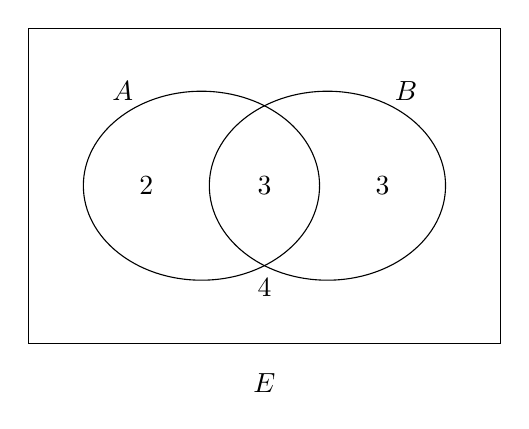
\begin{tikzpicture}
				% Hình chữ nhật biểu diễn tập E
				\draw (0,0) rectangle (6,4);
				\node at (3,-0.5) {$E$};
				
				% Hai hình elip biểu diễn tập A và B
				\draw (2.2,2) ellipse (1.5 and 1.2);
				\draw (3.8,2) ellipse (1.5 and 1.2);
				
				% Ghi nhãn tập A và B
				\node at (1.2,3.2) {$A$};
				\node at (4.8,3.2) {$B$};
				
				% Ghi các số vào từng vùng
				\node at (1.5,2) {$2$}; % chỉ thuộc A
				\node at (3,2) {$3$}; % giao A và B
				\node at (4.5,2) {$3$}; % chỉ thuộc B (chưa dùng đến)
				\node at (3,0.7) {$4$}; % ngoài A và B
		\end{tikzpicture}}
		Số học sinh tham gia tiết mục hát là $3 + 3 = 6$ (học sinh).
	}
\end{vd}
%%%=============================%%%

%%%=============VD_3=============%%%
\begin{vd}%[0D1V3-1]
	Lớp $10H$ có $37$ học sinh làm bài kiểm tra môn toán. Đề bài gồm có $3$ bài toán. Sau khi kiểm tra, cô giáo tổng hợp được kết quả như sau: có $20$ em giải được bài toán thứ nhất, $14$ em giải được bài toán thứ hai, $10$ em giải được bài toán thứ ba, $5$ em giải được bài toán thứ hai và thứ ba, $2$ em giải được bài toán thứ nhất và thứ hai, $6$ em giải được bài toán thứ nhất và thứ ba, chỉ có $1$ học sinh giải được cả ba bài toán. Hỏi lớp học đó có bao nhiêu học sinh không giải được bài toán nào?
	\loigiai{
		Gọi tập $A$ là tập hợp học sinh giải được câu $1$. Tập $A$ có $20$ phần tử.\\
		Gọi tập $B$ là tập hợp học sinh giải được câu $2$. Tập $B$ có $14$ phần tử.\\
		Gọi tập $C$ là tập hợp học sinh giải được câu $3$. Tập $C$ có $10$ phần tử.\\
		Gọi tập $A\cap B$ là tập hợp học sinh giải được câu $1$ và câu $2$. Tập $A\cap B$ có $2$ phần tử.\\
		Gọi tập $B\cap C$ là tập hợp học sinh giải được câu $2$ và câu $3$. Tập $B\cap C$ có $5$ phần tử.\\
		Gọi tập $A\cap C$ là tập hợp học sinh giải được câu $1$ và câu $3$. Tập $A\cap C$ có $6$ phần tử.\\
		Gọi tập $A\cap B\cap C$ là tập hợp học sinh giải được cả $3$ câu. Tập $A\cap B\cap C$ có $1$ phần tử.\\
		Áp dụng nguyên lý bù trừ ta có
		\begin{eqnarray*}
			&n(A\cup B\cup C)&=n(A)+n(B)+n(C)-n(A
			\cap B)-n(B\cap C)-n(A\cap C)+n(A\cap B\cap C)\\
			&&=20+14+10-2-5-6+1\\
			&&=32.
		\end{eqnarray*}
		Số học sinh không giải được bài toán nào là $37-32=5$ (học sinh).
	}
\end{vd}
%%%=============================%%%

\subsection{Bài tập rèn luyện}
\ind{PHẦN I.} \inden{Câu trắc nghiệm nhiều phương án lựa chọn. Mỗi câu hỏi học sinh chỉ chọn một phương án.}\\
\setcounter{ex}{0}
\Opensolutionfile{ans}[ans/0D1-Bai3-TN]

%%%=========EX_1=========%%%
\begin{ex}%[0D1N3-3]
	[\textit{GHKI NH23-24-THPT Hướng Hoá - Quảng Trị}]
	Cho hai tập hợp $A=(3 ; 6)$ và $B=(5 ; 8)$. Xác định tập hợp $C=A \cup B$.
	\choice
	{\True $C=(3 ; 8)$}
	{$C=(3 ; 5)$}
	{$C=(5 ; 6)$}
	{$C=(6 ; 8)$}
	\loigiai{
		Tập hợp $C=A \cup B=(3 ; 8)$.
	}
\end{ex}

%%%=========EX_2=========%%%
\begin{ex}%[0D1N3-1]
	[\textit{GHKI NH23-24-THPT Chu Văn An- Quảng Ngãi}]
	\immini{
		Cho tập hợp $A$, $B$ được biểu diễn bằng biểu đồ Ven như hình vẽ. Số phần tử của tập $A\cap B$ là
		\choice
		{$8$}
		{$5$}
		{$6$}
		{\True $3$}
	}
	{
		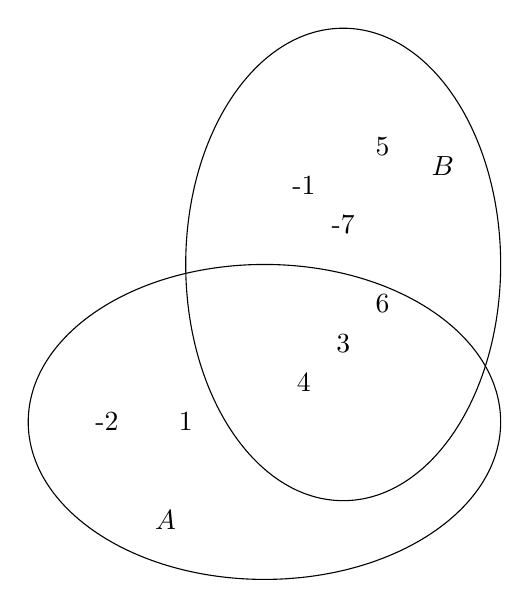
\begin{tikzpicture}
			\def\ElipA{(0,0) ellipse (3cm and 2cm)}
			\def\ElipB{(1,2) ellipse (2cm and 3cm)}
			\draw\ElipA node[black,below left=1cm] {$A$};
			\draw \ElipB node[black,above right=1cm] {$B$};
			\draw (1,1)node{3} (0.5,0.5)node{4} (1.5,1.5)node{6}
			(-1,0)node{1} (-2,0)node{-2}
			(1,2.5)node{-7} (0.5,3)node{-1} (1.5,3.5)node{5}
			;
		\end{tikzpicture}
	}
	\loigiai
	{
		Ta có $A\cap B=\{3;4;6\}$ nên số phần tử của $A\cap B$ là $3$.
	}
\end{ex}

%%%=========EX_3=========%%%
\begin{ex}%[0D1N3-4]
	Trong các hình minh họa bằng biểu đồ Ven dưới đây, phần gạch sọc trong hình nào là hình biểu diễn của tập hợp $A\cap B$ ?
	\choice
	{\True \begin{tikzpicture}[scale=.4,thick,rotate=-99]
			\colorlet{MauNet}{black}
			\def\ElipA{(0,0) ellipse (2cm and 3cm)}
			\def\ElipB{(1,3) ellipse (2cm and 3cm)}
			\begin{scope}
				\clip \ElipA;
				\fill[pattern=vertical lines,pattern color=black] \ElipB;
			\end{scope}
			\draw[MauNet] \ElipA node[black,below left=0.1cm] {$A$};
			\draw[MauNet] \ElipB node[black,above right=0.1cm] {$B$};
			\draw[MauNet] (current bounding box.north) node[black,anchor=south] {};
	\end{tikzpicture}}
	{\begin{tikzpicture}[scale=.4,thick,rotate=-99]
			\colorlet{MauNet}{black}
			\def\ElipA{(0,0) ellipse (2cm and 3cm)}
			\def\ElipB{(1,3) ellipse (2cm and 3cm)}
			\begin{scope}
				\clip \ElipA;
				\draw[MauNet,pattern=vertical lines,pattern color=black,even odd rule] \ElipA \ElipB;
			\end{scope}
			\draw[MauNet] \ElipA node[black,below left=0.1cm] {$A$} \ElipB node[black,above right=0.1cm]{$B$};
			\draw[MauNet] (current bounding box.north) node[black,anchor=south] {};
		\end{tikzpicture}
	}
	{\begin{tikzpicture}[scale=.4,thick,rotate=-99]
			\colorlet{MauNet}{black}
			\def\ElipA{(0,0) ellipse (2cm and 3cm)}
			\def\ElipB{(1,3) ellipse (2cm and 3cm)}
			\draw[MauNet,pattern=vertical lines,pattern color=black] \ElipA node[black,below left=0.1cm] {$A$} \ElipB node[black,above right=0.1cm]{$B$};
			\draw[MauNet] (current bounding box.north) node[black,anchor=south] {};
	\end{tikzpicture}}
	{\begin{tikzpicture}[scale=.4,thick,rotate=-99]
			\colorlet{MauNet}{black}
			\def\ElipA{(0,0) ellipse (2cm and 3cm)}
			\def\ElipB{(1,0.7) ellipse (0.7cm and 1.4cm)}
			\draw[MauNet,pattern=vertical lines,pattern color=black] \ElipA;
			\draw[MauNet,fill=white] \ElipB node[black]{$A$};
			\path[MauNet]\ElipA node[black]{$B$};
			\draw[MauNet] (current bounding box.north) node[black,anchor=south] {};
	\end{tikzpicture}}
	\loigiai{
		\immini
		{
			Dựa vào biểu đồ Ven ta thấy phần gạch sọc trong hình bên là hình biểu diễn của tập hợp $A\cap B$.
		}
		{
			\begin{tikzpicture}[scale=.4,thick,rotate=-99]
				\colorlet{MauNet}{black}
				\def\ElipA{(0,0) ellipse (2cm and 3cm)}
				\def\ElipB{(1,3) ellipse (2cm and 3cm)}
				\begin{scope}
					\clip \ElipA;
					\fill[pattern=vertical lines,pattern color=black] \ElipB;
				\end{scope}
				\draw[MauNet] \ElipA node[black,below left=0.1cm] {$A$};
				\draw[MauNet] \ElipB node[black,above right=0.1cm] {$B$};
				\draw[MauNet] (current bounding box.north) node[black,anchor=south] {};
			\end{tikzpicture}
		}
		}
\end{ex}

%%%=========EX_4=========%%%
\begin{ex}%[0D1N3-4]
	[\textit{HKI NH23-24-THPT Hồ Thị Bi}]
	Cho tập hợp $ A=\left [3;5\right )$. Khi đó $ C_{\mathbb{R}}A$ bằng tập hợp nào sau đây?
	\choice
	{$\left(-\infty;3\right]\cup \left[5;+\infty \right )$}
	{ $\left(-\infty;3\right]\cup \left(5;+\infty \right )$}
	{ $\left(-\infty;3\right)\cup \left(5;+\infty \right )$}
	{\True $\left(-\infty;3\right)\cup \left[5;+\infty \right )$}
	\loigiai{
		Ta có $C_{\mathbb{R}}A=\mathbb{R}\setminus A=\left(-\infty;3\right)\cup \left[5;+\infty \right )$.}
\end{ex}

%%%=========EX_5=========%%%
\begin{ex}%[0D1N3-4]
	[\textit{GHKI NH23-24-THPT Phan Châu Trinh - Đà Nẵng}]
	Cho $A=(-1;5]$, $B=(2;6]$. Tập hợp $A\setminus B$ là
	\choice
	{\True $(-1;2]$}
	{$(2;5)$}
	{$(1;2]$}
	{$(-1;6]$}
	\loigiai
	{
		\begin{center}
			\begin{tikzpicture}[scale=1, font=\footnotesize, line join=round, line cap=round,>=stealth]%<DTools>
				\def\xmin{-3};\def\xmax{8};
				%(-1;5]
				\draw[->] (\xmin,0)--(\xmax,0);
				\node (a0) at (-1,{0}){(};
				\node (b0) at (5,0){]};
				\draw (a0.-90)node[below]{$-1$} (b0.-90)node[below]{$5$};
				\draw[draw=none, pattern=north west lines] ($(a0)+(90:0.1)$)--(\xmin,0.1)--(\xmin,-0.1)--($(a0)+(-90:0.1)$) ($(b0)+(90:0.1)$)--(\xmax,0.1)--(\xmax,-0.1)--($(b0)+(-90:0.1)$);
				%(2;6]
				\draw[->] (\xmin,-1)--(\xmax,-1);
				\node (a1) at (2,{-1}){(};
				\node (b1) at (6,{-1}){]};
				\draw (a1.-90)node[below]{$2$} (b1.-90)node[below]{$6$};
				\draw[draw=none, pattern=north west lines] ($(a1)+(90:0.1)$)--(\xmin,{0.1-1})--(\xmin,{-0.1-1})--($(a1)+(-90:0.1)$) ($(b1)+(90:0.1)$)--(\xmax,{0.1-1})--(\xmax,{-0.1-1})--($(b1)+(-90:0.1)$);
			\end{tikzpicture}
		\end{center}
		Tập hợp $A\setminus B=\left(-1;2\right]$.
	}
\end{ex}

%%%=========EX_6=========%%%
\begin{ex}%[0D1H3-5]
	[\textit{HKI NH23-24 -THPT Mạc Đĩnh Chi}]
	Cho ba tập hợp $A=(1;+\infty)$, $B=(-2;3)$ và $C=[-5;2)$. Hãy tìm tập hợp $C\setminus (A \cup B)$.
	\choice
	{$(2;3)$}
	{$[-5;2)$}
	{\True $[-5;-2]$}
	{$(1;2)$}
	\loigiai{
		Ta có $A \cup B=(-2;+\infty) \Rightarrow C\setminus (A \cup B)=[-5;-2]$.
	}
\end{ex}

%%%=========EX_7=========%%%
\begin{ex}%[0D1H3-5]
	Một đoàn khách du lịch vào quán ăn sáng. Khi thanh toán tiền ăn, trưởng đoàn trả tiền cho $25$ tô bún bò, $16$ tô mì Quảng. Biết rằng mỗi khách ăn ít nhất một tô (bún hoặc mì) và có $7$ người ăn hai tô (một tô bún và một tô mì), không có ai ăn nhiều hơn hai tô. Hỏi đoàn khách đó có tất cả bao nhiêu người?
	\choice
	{$27$}
	{$41$}
	{\True $34$}
	{$48$}
	\loigiai{
		Gọi $A$và $B$ lần lượt là tập hợp các khách ăn một tô bún bò và một tô mì Quảng.\\
		Khi đó tập hợp khách ăn hai tô (một tô bún và một tô mì) là $A\cap B$.\\
		Đoàn khách du lịch đó có là $n(A\cup B)=n(A)+n(B)-n(A\cap B)=16+25-7=34$ (người).
	}
\end{ex}

%%%=========EX_8=========%%%
\begin{ex}%[0D1H3-5]
	[\textit{HKI NH23-24-THPT Chuyên Lê Quý Đôn-Ninh Thuận}]
	Để phục vụ cho một hội nghị quốc tế, ban tổ chức huy động 35 người phiên dịch tiếng Anh, 30 người phiên dịch tiếng Pháp, trong đó có 16 người phiên dịch được cả hai thứ tiếng Anh và tiếng Pháp. Hỏi ban tổ chức đã huy động bao nhiêu người phiên dịch cho hội nghị đó?
	\choice
	{$65$}
	{$19$}
	{\True $49$}
	{$14$}
	\loigiai{
		Số người phiên dịch cho hội nghị là $35+30-16=49$ (người).
	}
\end{ex}

%%%=========EX_9=========%%%
\begin{ex}%[0D1H3-5]
	[\textit{HKI NH23-24-THPT Trần Hưng Đạo}]
	Trong Kỳ thi tốt nghiệp phổ thông ở một trường, kết quả số thí sinh đạt danh hiệu xuất sắc như sau: về môn Toán: $48$ thí sinh; về môn Vật lý: $37$ thí sinh; về môn Văn: $42$ thí sinh; về môn Toán hoặc môn Vật lý: $75$ thí sinh; về môn Toán hoặc môn Văn: $76$ thí sinh; về môn Vật lý hoặc môn Văn: $66$ thí sinh; về cả $3$ môn: $4$ thí sinh. Vậy có bao nhiêu học sinh nhận được danh hiệu xuất sắc về một môn?
	\choice
	{$56$}
	{$47$}
	{$70$}
	{\True $65$}
	\loigiai{
		Gọi $x,y,z$ lần lượt là số học sinh chỉ đạt danh hiệu xuất sắc môn Toán, Vật lý và Văn $(x,y,z >0)$.\\
		Số học sinh đạt danh hiệu xuất sắc cả hai môn Toán và môn Vật lý là $48+37-75=10$.\\
		Số học sinh chỉ đạt danh hiệu xuất sắc hai môn Toán và môn Vật lý là $10-4=6$.\\
		Số học sinh đạt danh hiệu xuất sắc cả hai môn Toán và môn Văn là $48+42-76=14$.\\
		Số học sinh chỉ đạt danh hiệu xuất sắc hai môn Toán và môn Văn là $14-4=10$.\\
		Số học sinh đạt danh hiệu xuất sắc cả hai môn Văn và môn Vật lý là $42+37-66=13$.\\
		Số học sinh chỉ đạt danh hiệu xuất sắc hai môn Văn và môn Vật lý là $13-4=9$.\\
		\begin{center}
			\begin{tikzpicture}[scale=0.75]
				\draw (0,0) circle (3);
				\draw (3,0) circle (2.7);
				\draw (3,3) circle (2.7);
				\draw (1.8,-0.5) node{9}
				(4,-0.8)node{Văn}
				(4,-1.2)node[below]{$z $}
				(3.5,1.25)node{10}
				(3,4)node{Toán}
				(3,3.5)node[below]{$x$}
				(1.8,1.45)node{4}
				(1,2.3) node{$6$}
				(-1,0)node{Vật lý}
				(-1,-0.9)node{$y$};
			\end{tikzpicture}
		\end{center}
		Theo hình vẽ, số học sinh đạt danh hiệu xuất sắc môn Toán và Vật lý là $x+y+6+10+9+4$.\\ Do đó ta được $x+y+6+10+9+4=75 \Rightarrow x+y=46$. (1)\\
		Tiếp theo, số học sinh đạt danh hiệu xuất sắc môn Toán và Văn là $x+z+6+9+4+10$.\\ Do đó ta được $x+z+6+10+9+4=76 \Rightarrow x+z=47$. (2)\\
		Cuối cùng, số học sinh đạt danh hiệu xuất sắc môn Vật lý và Văn là $y+z+6+10+4+9$.\\ Do đó ta được $y+z+6+10+9+4=66 \Rightarrow y+z=37$. (3)\\
		Cộng $(1)$, $(2)$, $(3)$, ta được $$x+y+x+z+y+z=46+47+37 \Rightarrow 2(x+y+z)=130 \Rightarrow x+y+z=65.$$
		Vậy có $65$ học sinh nhận được danh hiệu xuất sắc về một môn.
	}
\end{ex}

%%%=========EX_10=========%%%
\begin{ex}%[0D1H3-1]
	[\textit{HKI NH23-24-THPT chuyên Lê Quý Đôn - Ninh Thuận}]
	Cho hai tập hợp $A=\left(-\infty;2024\right]$ và $B=\left(2024;+\infty \right)$. Khi đó $X=A\cup B$ bằng
	\choice
	{$\{2024\}$}
	{\True $\mathbb{R}$}
	{$\mathbb{R}\setminus \{2024\}$}
	{$\emptyset$}
	\loigiai{
		Ta có $A=\left(-\infty;2024\right]$ và $B=\left(2024;+\infty \right)$ nên $X=A\cup B=\mathbb{R}$.
	}
\end{ex}

%%%=========EX_11=========%%%
\begin{ex}%[0D1H3-1]
	[\textit{GHKI NH23-24 -THPT Vũ Duy Thanh}]
	Cho hai tập hợp $A$ và $B$ được mô tả bởi biểu đồ Ven sau đây.
	\begin{center}
		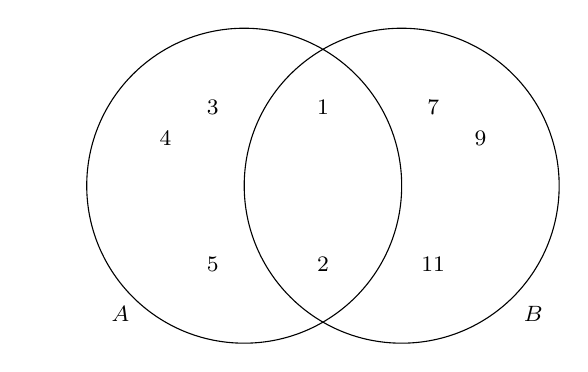
\begin{tikzpicture}[scale=1, font=\footnotesize, line join=round, line cap=round, >=stealth]
			\draw
			(-1,0) circle (2cm)
			(1,0) circle (2cm)
			;
			\path
			(0,1) node{$1$}
			(0,-1) node{$2$}
			(1.4,1) node{$7$}
			(2,0.6) node{$9$}
			(1.4,-1) node{$11$}
			(-1.4,1) node{$3$}
			(-2,0.6) node{$4$}
			(-1.4,-1) node{$5$}
			(-3.75,0)--++(-45:2) node[below left]{$A$}
			(1.5,0)--++(-45:2) node[below left]{$B$}
			;
		\end{tikzpicture}
	\end{center}
	Khẳng định nào sau đây là \textbf{đúng}?
	\choice
	{$A \cup B=\{3 ; 4 ; 5 ; 7 ; 9 ; 11\}$}
	{\True $A \cap B=\{1 ; 2\}$}
	{$B \setminus A=\{7 ; 9 ; 11\}$}
	{$A \setminus B=\{3 ; 4 ; 5\}$}
	\loigiai
	{
		Theo biểu đồ Ven thì $A\cap B=\{1;2\}$.
	}
\end{ex}

%%%=========EX_12=========%%%
\begin{ex}%[0D1H3-1]
	[\textit{GHKI NH23-24 -THPT Vũ Duy Thanh}]
	Cho hai tập hợp $A=\left\{x \in \mathbb{R} \mid\left(x^2-4 x\right)\left(2 x^2-3 x-2\right)=0\right\}$ và $B=\left\{n \in \mathbb{N} \mid 3<n^2<30\right\}$. Khi đó, $A \cap B$ là?
	\choice
	{$\{3\}$}
	{$\{2\}$}
	{$\{5 ; 4\}$}
	{\True $\{2 ; 4\}$}
	\loigiai
	{
		Ta giải phương trình
		\begin{align*}
			\left(x^2-4 x\right)\left(2 x^2-3 x-2\right)=0&\Leftrightarrow \hoac{
				&x^2-4x=0\\
				&2x^2-3x-2=0}\Leftrightarrow\hoac{&x=0\\&x=4\\&x=2\\&x=-\dfrac{1}{2}.}
		\end{align*}
		Do đó $A=\left\{-\dfrac{1}{2};0;2;4\right\}$.\\
		Vì $n\ge0$ nên ta có
		\begin{align*}
			3<n^2<30\Leftrightarrow \sqrt{3}<n<\sqrt{30}.
		\end{align*}
		Do đó $B=\left\{2;3;4;5\right\}$.\\
		Vậy $A\cap B=\{2;4\}$.
	}
\end{ex}

%%%=========EX_13=========%%%
\begin{ex}%[0D1H3-1]
	[\textit{GHKI NH23-24-THPT Chu Văn An - Quảng Ngãi}]
	Cho hai tập hợp $A = \left\lbrace 1; 2; 3 \right\rbrace$ và $B = \left\lbrace 0; 2; 3; 6 \right\rbrace$. Tập $A \cap B$ bằng
	\choice
	{$\left\lbrace 0; 1; 2; 3; 6 \right\rbrace $}
	{$\left\lbrace 0; 6 \right\rbrace $}
	{$\left\lbrace 1 \right\rbrace $}
	{\True $\left\lbrace 2; 3 \right\rbrace $}
	\loigiai{
		Ta có $A \cap B = \left\lbrace 2; 3 \right\rbrace $.
	}
\end{ex}

%%%=========EX_14=========%%%
\begin{ex}%[0D1H3-4]
	[\textit{GHKI NH23-24-Chuyên Lê Quý Đôn - Bình Định}]
	Cho $A=(6;+\infty)$. Khi đó $\mathrm{C}_\mathbb{R}A$ là tập nào sau đây?
	\choice
	{$\mathrm{C}_\mathbb{R}A=\{6\}$}
	{\True $\mathrm{C}_\mathbb{R}A=(-\infty;6]$}
	{$\mathrm{C}_\mathbb{R}A=(6; +\infty)$}
	{$\mathrm{C}_\mathbb{R}A=(-\infty;6)$}
	\loigiai{
		Ta có $\mathrm{C}_\mathbb{R}A=(-\infty;6]$.
	}
\end{ex}

%%%=========EX_15=========%%%
\begin{ex}%[0D1H3-4]
	[\textit{HKI NH23-24-THPT Lê Thánh Tôn}]
	Cho hai tập hợp $A=\{x\in\mathbb{Z}\colon -4<x\leq 4\}$ và $B=\{x\in \mathbb{Q}\colon x^2-16=0\}$. Tập hợp $B\setminus A$ bằng
	\choice
	{$\varnothing$}
	{$\{4\}$}
	{\True $\{-4\}$}
	{$\{-4;4\}$}
	\loigiai{
		Ta có $A=\{-3;-2;-1;0;1;2;3;4\}$.\\
		Do $x^2-16=0\Leftrightarrow x=\pm 4$ nên $B=\{-4;4\}$.\\
		Vậy $B\setminus A=\{-4\}$.
	}
\end{ex}

%%%=========EX_16=========%%%
\begin{ex}%[0D1H3-4]
	[\textit{GHKI NH23-24-THPT Chuyên Lê Khiết}]
	Cho hai tập hợp $A= [-1;3)$ và $B=(2;5]$. Khẳng định nào sau đây {\bf sai}?
	\choice
	{\True $B \setminus A= (3;5]$}
	{$A \cap B=(2;3)$}
	{$A \cup B=[-1;5]$}
	{$A \setminus B= [-1;2]$}
	\loigiai{
		Cho hai tập hợp $A= [-1;3)$ và $B=(2;5]$.\\
		Khi đó
		$A \cap B=(2;3)$; $A \cup B=[-1;5]$; $B \setminus A= [3;5]$; $A \setminus B= [-1;2]$.\\
		Khẳng định sai là $B \setminus A= (3;5]$.
	}
\end{ex}

%%%=========EX_17=========%%%
\begin{ex}%[0D1H3-4]
	[\textit{GHKI - THPT Ngô Quyền - Đồng Nai}]
	Cho tập hợp $A=(-3 ; 4]$. Xác định tập hợp $\mathrm{C}_{\mathbb{R}} A$.
	\choice
	{$(-\infty ;-3) \cup(4 ;+\infty)$}
	{\True $(-\infty ;-3] \cup(4 ;+\infty)$}
	{$(-\infty ;-3] \cup[4 ;+\infty)$}
	{$(-\infty ;-3) \cup[4 ;+\infty)$}
	\loigiai{
		$\mathrm{C}_{\mathbb{R}} A=\mathbb{R}\setminus A=\left(-\infty;-3\right]\cup \left(4;+\infty\right)$.
	}
\end{ex}

%%%=========EX_18=========%%%
\begin{ex}%[0D1H3-4]
	[\textit{GHKI NH23-24-THPT Phan Châu Trinh - Đà Nẵng}]
	Cho $C_{\mathbb{R}}A=[-3;+\infty)$. Tập hợp $A$ bằng
	\choice
	{$(-\infty;3)$}
	{\True$(-\infty;-3)$}
	{$(-\infty;-3]$}
	{$(-\infty;3]$}
	\loigiai
	{ Vì $C_{\mathbb{R}}A=[-3;+\infty)$ nên tập hợp $A=\left(-\infty;-3\right)$.
	}
\end{ex}

%%%=========EX_19=========%%%
\begin{ex}%[0D1H3-4]
	[\textit{GHK1 lớp 10 NH23-24-THPT Thanh Miện 2}]
	Cho $A=(-\infty ; 3] ; B=[2 ;+\infty)$ và $C=(0 ; 4)$. Khi đó tập $(A \cup B) \backslash C$ là
	\choice
	{$[3 ; 4]$}
	{$(-\infty ;-2) \cup[3 ;+\infty)$}
	{$(3 ; 4)$}
	{\True $(-\infty ; 0] \cup[4 ;+\infty)$}
	\loigiai{
		Ta có $A \cup B=\left(-\infty;+\infty\right)$.\\
		Suy ra $(A\cup B)\backslash C=(-\infty ; 0] \cup[4 ;+\infty)$.
	}
\end{ex}

%%%=========EX_20=========%%%
\begin{ex}%[0D1H3-5]
	Một đoàn khách du lịch vào quán ăn sáng. Khi thanh toán tiền ăn, trưởng đoàn trả tiền cho $25$ tô bún bò, $16$ tô mì Quảng. Biết rằng mỗi khách ăn ít nhất một tô (bún hoặc mì) và có $7$ người ăn hai tô (một tô bún và một tô mì), không có ai ăn nhiều hơn hai tô. Hỏi đoàn khách đó có tất cả bao nhiêu người?
	\choice
	{$27$}
	{$41$}
	{\True $34$}
	{$48$}
	\loigiai{
		Gọi $A$và $B$ lần lượt là tập hợp các khách ăn một tô bún bò và một tô mì Quảng.\\
		Khi đó tập hợp khách ăn hai tô (một tô bún và một tô mì) là $A\cap B$.\\
		Đoàn khách du lịch đó có  là $n(A\cup B)=n(A)+n(B)-n(A\cap B)=16+25-7=34$ (người).
	}
\end{ex}
\Closesolutionfile{ans}

\ind{PHẦN II.} \inden{Câu trắc nghiệm đúng sai. Trong mỗi ý a), b), c), d) ở mỗi câu, học sinh chọn đúng hoặc sai.}\\
\setcounter{ex}{0}
\Opensolutionfile{ans}[ans/0D1-Bai3-DS]
%%%=============EX_1=============%%%
\begin{ex}%[0D1H3-2]
	Cho hai tập hợp $A=\left\{0;1;2;3;4\right\}$, $B=\left\{3;4;5;6\right\}$.
	\choiceTF
	{\True $A\cup B=\left\{0;1;2;3;4;5;6\right\}$}
	{$A\cap B=\left\{5;6\right\}$}
	{$B\setminus A=\left\{0;1;2\right\}$}
	{\True $\left(A\cup B\right)\setminus \left(A\cap B\right)=\left(A\setminus B\right)\cup \left(B\setminus A\right)$}
	\loigiai{
		\begin{itemchoice}
			\itemch Ta có $A\cup B=\left\{0;1;2;3;4;5;6\right\}$.
			\itemch Ta có $A\cap B=\left\{3;4\right\}$.
			\itemch Ta có $B\setminus A=\left\{5;6\right\}$.
			\itemch Ta có $A\cup B=\left\{0;1;2;3;4;5;6\right\}$, $A\cap B=\left\{3;4\right\}$ nên $\left(A\cup B\right)\setminus \left(A\cap B\right)=\left\{0;1;2;5;6\right\}$.\\
			Ta có $A\setminus B=\left\{0;1;2\right\}$, $B\setminus A=\left\{5;6\right\}$ nên $\left(A\setminus B\right)\cup \left(B\setminus A\right)$ $=\left\{0;1;2;5;6\right\}$.
		\end{itemchoice}
	}
\end{ex}
%%%=============================%%%

%%%=============EX_2=============%%%
\begin{ex}%[0D1H3-2]
	Cho ba tập hợp $A = \{x \in \mathbb{Z} \mid -3 \leq x \leq 4\}$, $B = \{x \in \mathbb{Z} \mid x < 2\}$, $C = \{x \in \mathbb{Z} \mid x \geq 0\}$.
	\choiceTF
	{$(A \cap B) \cup C = A$}
	{\True $A \cap (B \cup C) = A$}
	{\True $A \cup (B \cap C) = A$}
	{\True $(A \setminus B) \cap C = \{2;3;4\}$}
	\loigiai
	{Ta có $A = \{-3;-2;-1;0;1;2;3;4\}$, $B = \{\ldots;-2;-1;0;1\}$, $C = \{0;1;2;3;\ldots\}$.
		\begin{itemchoice}
			\itemch Ta có $A \cap B = \{-3;-2;-1;0;1\}$ $\Rightarrow$ $(A \cap B) \cup C = \{-3;-2;-1;0;1;2;3;4;\ldots\} \neq A$.
			\itemch Ta có $B \cup C = \mathbb{Z}$ nên $A \cap (B \cup C) = A$.
			\itemch Ta có $B \cap C = \{0;1\}$, $A \cup (B \cap C) = A$.
			\itemch Ta có $A \setminus B = \{2;3;4\}$, giao với $C$ vẫn là $\{2;3;4\}$.
		\end{itemchoice}
	}
\end{ex}
%%%=============================%%%

%%%=============EX_3=============%%%
\begin{ex}%[0D1V2-1]
	Lớp $10A$ có $26$ học sinh biết chơi đá bóng, $22$ học sinh biết chơi cầu lông, $5$ học sinh biết chơi cả hai môn đá bóng và cầu lông, $8$ học sinh không biết chơi môn nào.
	\choiceTF
	{\True Số học sinh chỉ biết chơi cầu lông mà không biết chơi đá bóng là $17$}
	{Số học sinh chỉ biết chơi đá bóng mà không biết chơi cầu lông là $20$}
	{\True Số học sinh biết chơi ít nhất một trong hai môn đá bóng hoặc cầu lông là $43$}
	{Sĩ số lớp $10A$ là $61$}
	\loigiai{
		\begin{center}
			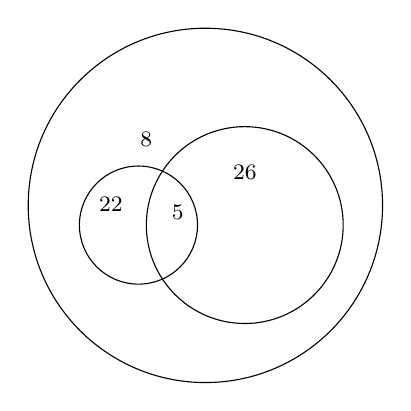
\begin{tikzpicture}[smooth,font=\footnotesize,scale=0.5]
				\draw[black] (0,0) circle (4.5cm);
				\draw[black] (-1.7,-.5) circle (1.5cm);
				\draw[black] (1.0,-.5) circle (2.5cm);
				\node at (-1.5,1.25)[above]{$8$};
				\node at (-.7,-0.6)[above]{$5$};
				\node at (1,0.4)[above]{$26$};
				\node at (-2.4,-0.4)[above]{$22$};
			\end{tikzpicture}
		\end{center}
		Dựa vào sơ đồ ven ta suy ra
		\begin{itemchoice}
			\itemch Số học sinh chỉ biết chơi cầu lông mà không biết chơi đá bóng là $22-5=17$.
			\itemch Số học sinh chỉ biết chơi đá bóng mà không biết chơi cầu lông là $26-5=21$
			\itemch Số học sinh biết chơi ít nhất một trong hai môn đá bóng hoặc cầu lông là $\left(22+26\right)-5=43$.
			\itemch Sĩ số lớp $10A$ là $22+26-5+8=51$.
		\end{itemchoice}
	}
\end{ex}
%%%=============================%%%

%%%=============EX_4=============%%%
\begin{ex}%[0D1V3-4]
	Cho các tập hợp $A=[-3;1)$, $B=[0;5)$, $C=[a;a+3]$.
	\choiceTF
	{$A\cup B=[0;1)$}
	{$A\cap B=[-3;5)$}
	{\True $B\setminus A=[1;5)$}
	{\True $A\cap C\neq \varnothing \Leftrightarrow$ $-6\leq a < 1$}
	\loigiai{
		\begin{itemchoice}
			\itemch Ta có $A\cup B=[-3;5)$.
			\itemch Ta có $A\cap B=[0;1)$.
			\itemch Ta có $B\setminus A=[1;5)$.
			\itemch Ta có $A\cap C=\varnothing$ khi
			\begin{itemize}
				\item TH1: $a+3<-3$ hay $a <-6. \quad(1)$
				\item TH2: $a\geq 1. \quad(2)$
			\end{itemize}
			Từ (1) và (2) suy ra $A\cap C\neq \varnothing$ khi $-6\leq a < 1$.
		\end{itemchoice}
	}
\end{ex}
%%%=============================%%%

%%%=============EX_5=============%%%
\begin{ex}%[0D1V3-4]
	Cho ba tập hợp $A=\left(1;\dfrac{11}{2} \right)$; $B=\left[-2;3\right]$ và $C=\left(\dfrac{m-1}{3};+\infty \right)$.
	\choiceTF
	{\True Giao của hai tập hợp $A$ và $B$ là $\left(1; 3\right]$}
	{Tập hợp $B\cap \mathbb{N}$ gồm $6$ phần tử}
	{\True Tập hợp $\mathbb{R}\setminus A=\left(-\infty;1\right]\cup \left[\dfrac{11}{2};+\infty \right)$}
	{\True Tổng các giá trị nguyên của $m$ để $B\cap C$ có đúng $3$ phần tử là số nguyên bằng $6$}
	\loigiai{
		\begin{itemchoice}
			\itemch Ta biểu diễn hai tập hợp $A$ và $B$ trên trục số.
			\begin{center}
				\begin{tikzpicture}[>=stealth,line join=round,line cap=round,font=\footnotesize,scale=1]
					\node at (-5,0)[left]{A};
					\draw[->,black] (-4,0)--(9.1,0);
					\path (1,0)node[]{$($}node[below=5pt]{$1$} (5.5,0)node[]{$]$}node[below=5pt]{$\dfrac{11}{2}$};
					\path[pattern=north west lines,pattern color=blue] (-4,-5pt)rectangle(1,3pt) (5.5,-3pt)rectangle(9,3pt);
				\end{tikzpicture}
			\end{center}
			\begin{center}
				\begin{tikzpicture}[>=stealth,line join=round,line cap=round,font=\footnotesize,scale=1]
					\node at (-5,0)[left]{B};
					\draw[->,black] (-4,0)--(9.1,0);
					\path (-2,0)node[]{$[$}node[below=5pt]{$-2$}
					(3,0)node[]{$]$}node[below=5pt]{$3$};
					\path[pattern=north west lines,pattern color=blue] (-4,-3pt)rectangle(-2,3pt)(3,-3pt)rectangle(9,3pt);
				\end{tikzpicture}
			\end{center}
			Suy ra $A\cap B=\left(1; 3\right]$.
			\itemch Vì $B\cap \mathbb{N}=\left\{0; 1; 2; 3\right\}$ $\Rightarrow n\left(B\cap \mathbb{N}\right)=4$.
			\itemch Ta có sự biểu diễn tập hợp $A$.
			\begin{center}
				\begin{tikzpicture}[>=stealth,line join=round,line cap=round,font=\footnotesize,scale=1]
					\node at (-5,0)[left]{A};
					\draw[->,black] (-4,0)--(9.1,0);
					\path (1,0)node[]{$($}node[below=5pt]{$1$} (5.5,0)node[]{$)$}node[below=5pt]{$\dfrac{11}{2}$};
					\path[pattern=north west lines,pattern color=blue] (-4,-5pt)rectangle(1,3pt) (5.5,-3pt)rectangle(9,3pt);
				\end{tikzpicture}
			\end{center}
			Suy ra $\mathbb{R}\setminus A=\left(-\infty;1\right]\cup \left[\dfrac{11}{2};+\infty \right)$.
			\itemch Để $B\cap C$ có đúng $3$ phần tử là số nguyên $\Leftrightarrow 0\leq \dfrac{m-1}{3} < 1\Leftrightarrow 1\leq m< 4$.\\
			Mà $m\in \mathbb{Z}\Rightarrow m\in \left\{1; 2; 3\right\}$.\\ Tổng các giá trị nguyên của $m$ là $1+2+3=6$.
		\end{itemchoice}
	}
\end{ex}
%%%=============================%%%
\Closesolutionfile{ans}


\ind{PHẦN III.} \inden{Câu trắc nghiệm trả lời ngắn.}
\setcounter{ex}{0}
\Opensolutionfile{ans}[ans/0D1-Bai3-TLN]
%%%=============EX_1=============%%%
\begin{ex}%[0D1V3-3]
	Cho tập hợp $A=\left\{x\in \mathbb{R}\mid \left(2x-11\right)\left(x^2+3\right)\leq 0\right\}$. Số phần tử của $A\cap \mathbb{N}$ bằng bao nhiêu?
	\par
	\shortans[oly]{6}
	\loigiai{
		Xét bất phương trình $\left(2x-11\right)\left(x^2+3\right)\leq 0\Leftrightarrow 2x-11\leq 0\Leftrightarrow x\leq \dfrac{11}{2}$
		\[\Rightarrow A=\left(-\infty; \dfrac{11}{2} \right]\Rightarrow A\cap \mathbb{N}=\left\{0; 1; 2; 3; 4;5\right\}.
		\]
		Suy ra số phần tử của $A\cap \mathbb{N}$ bằng $6$.
	}
\end{ex}
%%%=============================%%%

%%%=============EX_2=============%%%
\begin{ex}%[0D1V3-1]
	Cho các tập hợp
	\begin{eqnarray*}
		&&A=\left\{x\in \mathbb{Q}\mid (x-1)(3x-2)(x+\sqrt{2} )=0\right\}\\
		&&B=\left\{x\in \mathbb{R}\mid (2+x)(3x-m^2+4)=0\right\}.
	\end{eqnarray*}
	Tích các giá trị của tham số $m$ để $n(A\cup B)=3$ bằng bao nhiêu?
	\par
	\shortans[oly]{42}
	\loigiai{
		Xét các phương trình
		\begin{itemize}
			\item $\left(x-1\right)\left(3x-2\right)\left(x+\sqrt{2} \right)=0\Leftrightarrow \hoac{&x=1\in \mathbb{Q}\\&x=\dfrac{2}{3} \in \mathbb{Q}\\&x=-\sqrt{2} \notin \mathbb{Q}}\Rightarrow A=\left\{1; \dfrac{2}{3} \right\}$.
			\item $\left(2+x\right)\left(3x-m^2+4\right)=0\Leftrightarrow \hoac{&x=-2\\&x=\dfrac{m^2-4}{3}.}$
		\end{itemize}
		Ta thấy $m^2 \geq 0$, $\forall m\Rightarrow \dfrac{m^2-4}{3} \ge-\dfrac{4}{3}$, $\forall m\Rightarrow-2\neq \dfrac{m^2-4}{3}$ $\Rightarrow B=\left\{\dfrac{m^2-4}{3};-2\right\}$.\\ Khi đó $n\left(A\cup B\right)=3$ $\Leftrightarrow \hoac{&\dfrac{m^2-4}{3}=1\\& \dfrac{m^2-4}{3}=\dfrac{2}{3}\\&\dfrac{m^2-4}{3}=-2}\Leftrightarrow \hoac{&m=\pm \sqrt{7}\\&m=\pm \sqrt{6}.}$\\ Suy ra tích các giá trị của tham số $m$ là $-\sqrt{7}\cdot \sqrt{7}\cdot \left(-\sqrt{6} \right)\cdot \sqrt{6}=42$.
	}
\end{ex}
%%%=============================%%%

%%%=============EX_3=============%%%
\begin{ex}%[0D1C2-1]
	Một lớp có $45$ học sinh, đăng kí chơi ít nhất một trong hai môn thể thao là bóng đá và cầu lông. Có $30$ em đăng kí môn bóng đá, $25$ em đăng kí môn cầu lông. Hỏi có bao nhiêu em đăng kí cả hai môn thể thao?
	\par
	\shortans[oly]{10}
	\loigiai{
		\begin{itemize}
			\item Gọi $A$ là tập hợp các bạn đăng ký môn bóng đá, $B$ là tập hợp các bạn đăng kí cầu lông.
			\item Số học sinh của lớp là
			\begin{eqnarray*}
				&&n(A\cup B)=n(A)+n(B)-n(A\cap B)\\
				&\Leftrightarrow&45=25+30-n(A\cap B)\\
				&\Leftrightarrow&n(A\cap B)=10.
			\end{eqnarray*}
		\end{itemize}
		Vậy có $10$ bạn đăng ký cả hai môn.
	}
\end{ex}
%%%=============================%%%

%%%=============EX_4=============%%%
\begin{ex}%[0D1C2-1]
	Lớp $10$A có $45$ học sinh trong đó có $25$ em học sinh học giỏi môn Toán, $23$ em học sinh học giỏi môn Văn, $20$ em học sinh học giỏi môn Tiếng Anh. Đồng thời có $11$ em học sinh học giỏi cả môn Toán và môn Văn, $8$ em học sinh học sinh giỏi cả môn Văn và môn Tiếng Anh, $9$ em học sinh học giỏi cả môn Toán và môn Tiếng Anh, biết rằng mỗi học sinh trong lớp học giỏi ít nhất một trong ba môn Toán, Văn, Tiếng Anh. Hỏi lớp 10A có bao nhiêu bạn học giỏi cả ba môn Toán, Văn, Tiếng Anh?
	\par
	\shortans[oly]{5}
	\loigiai{
		\begin{center}
			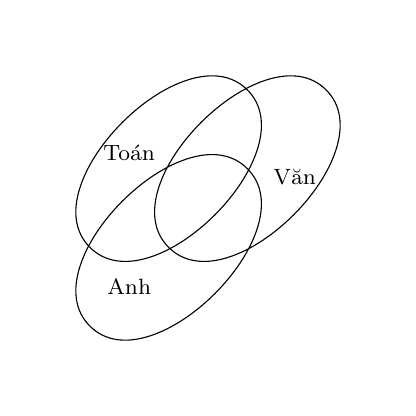
\begin{tikzpicture}[smooth,font=\footnotesize,scale=1.0]
				\def\miena{(0,0) to[bend left=90] (2,2) to[bend left=90] (0,0)}
				\def\mienb{(1,0) to[bend left=90] (3,2) to[bend left=90] (1,0)}
				\def\mienc{(0,-1) to[bend left=90] (2,1) to[bend left=90] (0,-1)}
				\draw \miena \mienb \mienc
				(0.5,1.2) node{Toán}
				(2.6,0.9) node{Văn}
				(0.5,-0.5) node{Anh};
			\end{tikzpicture}
		\end{center}
		Gọi $x$ ($x\in \mathbb{N}$) là số học sinh giỏi cả ba môn Toán, Văn, Anh.\\
		Số học sinh chỉ giỏi Toán và Văn là $11-x$ (học sinh).\\
		Số học sinh chỉ giỏi Toán và Anh là $9-x$ (học sinh).\\
		Số học sinh chỉ giỏi Văn và Anh là $8-x$ (học sinh).\\
		Số học sinh chỉ giỏi Toán là $25-\left(11-x\right)-\left(9-x\right)-x=5+x$ (học sinh).\\
		Số học sinh chỉ giỏi Văn là $23-\left(11-x\right)-\left(8-x\right)-x=4+x$ (học sinh).\\
		Số học sinh chỉ giỏi Anh là $20-\left(9-x\right)-\left(8-x\right)-x=3+x$ (học sinh).\\
		Lớp có $45$ học sinh nên ta có
		\begin{eqnarray*}
			&&x+\left(11-x\right)+\left(9-x\right)+\left(8-x\right)+5+x+4+x+3+x=45\\
			&\Leftrightarrow& x+40=45\\
			&\Leftrightarrow& x=5.
		\end{eqnarray*}
		Vậy có $5$ học sinh giỏi cả ba môn Toán, Văn và Anh.
	}
\end{ex}
%%%=============================%%%

%%%=============EX_5=============%%%
\begin{ex}%[0D1C2-2]
	Cho hai tập hợp $A=\left\{x\in \mathbb{R}\mid 1\leq \left|x\right|\leq 2\right\}$; $B=\left(-\infty;m-2\right]\cup \left[m;+\infty \right)$. Có bao nhiêu giá trị nguyên của $m\in [-2023;2024]$ để $A\subset B$?
	\par
	\shortans[oly]{4044}
	\loigiai{
		\begin{center}
			\begin{tikzpicture}[>=stealth,line join=round,line cap=round,font=\footnotesize,scale=1]
				\node at (-5,0)[left]{A};
				\draw[->,black] (-4,0)--(9.1,0);
				\path (-2,0)node[]{$[$}node[below=5pt]{$-2$} (-1,0)node[]{$]$}node[below=5pt]{$-1$};
				\path[pattern=north west lines,pattern color=blue] (-4,-5pt)rectangle(-2,3pt) (-1,-3pt)rectangle(1,3pt);
				\path (1,0)node[]{$[$}node[below=5pt]{$1$} (2,0)node[]{$]$}node[below=5pt]{$2$};
				\path[pattern=north west lines,pattern color=blue] (-1,-5pt)rectangle(1,3pt) (2,-3pt)rectangle(9,3pt);
			\end{tikzpicture}
		\end{center}
		\begin{center}
			\begin{tikzpicture}[>=stealth,line join=round,line cap=round,font=\footnotesize,scale=1]
				\node at (-5,0)[left]{B};
				\draw[->,black] (-4,0)--(9.1,0);
				\path (-1,0)node[]{$]$}node[below=5pt]{$m-2$} (1,0)node[]{$[$}node[below=5pt]{$m$};
				\path[pattern=north west lines,pattern color=blue] (-1,-5pt)rectangle(1,3pt);
			\end{tikzpicture}
		\end{center}
		Giải bất phương trình $1\leq \left|x\right|\leq 2\Leftrightarrow x\in \left[-2;-1\right]\cup \left[1;2\right]$
		\[\Rightarrow A=\left[-2;-1\right]\cup \left[1;2\right].
		\]
		Để $A\subset B$ ta cần có $\hoac{&m-2\geq 2\\&m\le-2\\&\heva{&-1\leq m-2\\&m\leq 1}} \Leftrightarrow \hoac{& m\geq 4\\&m\leq-2\\&m=1.}$\\
		Mà $m$ nguyên và $m\in [-2\,023;2\,024]$ nên $m\in \left\{-2\,023;-2\,022;\ldots;-2;1;4;5;\ldots;2\,024\right\}$.\\
		Vậy có $-2-(-2\,023)+1+1+2\,024-4+1=4\,044$.
	}
\end{ex}
%%%=============================%%%

\Closesolutionfile{ans}


\ind{PHẦN IV.} \inden{Tự luận.}\\
\setcounter{ex}{0}
%%%=============EX_1=============%%%
\begin{ex}%[0D1H3-3]
	[\textit{GHKI NH23-24-Sở GDĐT Bắc Ninh}]
	Cho các tập hợp
	\begin{eqnarray*}
		&&A=\left \{x\in\mathbb{R}\,|\,2x-1<9 \right \}, B=\left \{x\in\mathbb{R}\,|\,-10\leq x\leq 10 \right\}.
	\end{eqnarray*}
	\begin{enumerate}
		\item Viết các tập hợp $A$, $B$ dưới dạng khoảng, nửa khoảng hay đoạn, rồi biểu diễn chúng trên trục số.
		\item Xác định các tập hợp $A\cap B$, $A\cup B$.
	\end{enumerate}
	\loigiai
	{
		\begin{enumerate}
			\item Ta có $2x-1<9\Leftrightarrow x<5$. Khi đó $A=(-\infty ;5)$.\\
			Lại có $-10\leq x\leq 10$. Khi đó $B=[-10;10]$.\\
			Biểu diễn tập hợp $A=(-\infty ;5)$ và $B=[-10;10]$ trên trục số ta được
			\begin{center}
				\begin{tikzpicture}[scale=1,>=stealth, font=\footnotesize,line join=round,line cap=round]
					\def\xmin{-5}\def\xmax{5}
					\node at (\xmin-2.5,0)[right]{$A=(-\infty ;5)$};
					\draw[->] (\xmin,0)--(\xmax,0);
					\node at (\xmin-2.5,-1)[right]{$B=[-10;10]$};
					\draw[->] (\xmin,-1)--(\xmax,-1);
					\path (1.5,0)node[shift={(90:5mm)}]{$5$}(1.5,0)node{$\big)$};
					\fill[pattern=north west lines]
					(\xmax-0.2,-0.1) rectangle (1.5,0.1);
					\path (-2,-1)node[shift={(90:5mm)}]{$-10$}(-2,-1)node{$\big[$}
					(\xmax,-1)node[shift={(90:5mm)}]{$+\infty$}
					;
					\fill[pattern=north west lines]
					(\xmin,-1.1) rectangle (-2,-0.9)
					;
					\path (3,-1)node[shift={(90:5mm)}]{$10$}(3,-1)node{$\big]$};
					\fill[pattern=north west lines]
					(\xmax-0.2,-1.1) rectangle (3,-0.9);
				\end{tikzpicture}
			\end{center}
			\item Ta có $A\cap B=[-10;5)$ và $A\cup B=(-\infty ;10]$.
		\end{enumerate}
	}
\end{ex}
%%%=============================%%%

%%%=============EX_2=============%%%
\begin{ex}%[0D1H3-3]
	[\textit{HKI NH23-24-THPT Trần Khai Nguyên- Tp HCM}]
	Cho các tập hợp 
	\begin{eqnarray*}
		&&A = \{x \in \mathbb{R} \mid -4 \leq x \leq 4\};
		B = \{x \in \mathbb{R} \mid 5 - 2x > 0\}.
	\end{eqnarray*}
	\begin{enumerate}
		\item Dùng các kí hiệu đoạn, khoảng, nửa khoảng để viết lại tập hợp $A$ và tập hợp $B$.
		\item Xác định các tập hợp $A \cap B$, $A \cup B$, $C_{\mathbb{R}} A$.
	\end{enumerate}
	\loigiai{
		\begin{enumerate}
			\item Ta có $A=\left[-4;4\right]$.\\
			Xét $5-2x>0 \Leftrightarrow -2x>-5 \Leftrightarrow x<\dfrac{5}{2}$. Vậy $B=\left(-\infty;\dfrac{5}{2}\right)$.
			\item $A \cap B=\left[-4;\dfrac{5}{2}\right)$.\\
			$A \cup B=\left(-\infty;4\right]$.\\
			$C_{\mathbb{R}}A=\left(-\infty;-4\right) \cup \left(4;+\infty\right)$.
		\end{enumerate}
	}
\end{ex}
%%%=============================%%%

%%%=============EX_3=============%%%
\begin{ex}%[0D1H3-3]
	[\textit{GHKI NH23-24-THPT Trần Hưng Đạo - Đắk Lắk}]
	Cho hai tập hợp 
	\begin{eqnarray*}
		&&A = \{x \in \mathbb{R} | 3 < x \leq 10 \};
		B = \{ x \in \mathbb{R} | x \geq 5\}.
	\end{eqnarray*}
	\begin{listEX}[1]
		\item Viết các tập hợp sau dưới dạng khoảng, đoạn, nửa khoảng trong $\mathbb{R}$.
		\item Tìm và biểu diễn trên trục số các tập hợp sau $A \cup B$, $A \cap B$, $A \backslash B$.
	\end{listEX}
	\loigiai{
		\begin{listEX}[1]
			\item $A = (3;10]$, $B = [5; +\infty)$.
			\item 
			\immini{$A \cup B = (3;+\infty)$}{\begin{tikzpicture}
					\draw[-stealth] (0,0)--(10.5,0) node[above]{$x$};
					\path
					(3,-.15) node[below]{$3$}
					(5,-.15) node[below]{$5$}
					(10,-.15) node[below]{$10$} 
					(3,0) node{$($}
					(5,0) node{$[$}
					(10,0) node{$]$}
					;
					\foreach \x in {0,.1,...,3} \draw(\x-.05,-.05)--(\x+.05,.05);
					%\foreach \x in {-1,...,10} \draw (\x,-.05)--(\x,.05);
			\end{tikzpicture}}
			\immini{$A \cap B = [5;10]$}{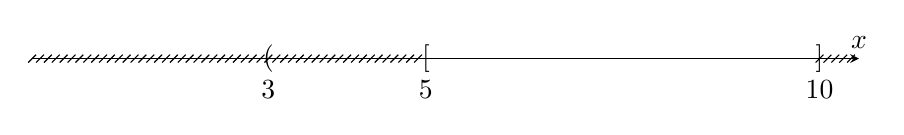
\begin{tikzpicture}
					\draw[-stealth] (0,0)--(10.5,0) node[above]{$x$};
					\path 
					(3,-.15) node[below]{$3$}
					(5,-.15) node[below]{$5$}
					(10,-.15) node[below]{$10$} 
					(3,0) node{$($}
					(5,0) node{$[$}
					(10,0) node{$]$}
					;
					\foreach \x in {0,.1,...,5} \draw(\x-.05,-.05)--(\x+.05,.05);
					\foreach \x in {10,10.1,...,10.42} \draw(\x-.05,-.05)--(\x+.05,.05);
					%\foreach \x in {-1,...,10} \draw (\x,-.05)--(\x,.05);
			\end{tikzpicture}}
			\immini{$A \backslash B = (3;5)$}{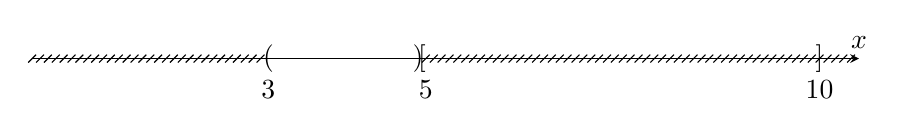
\begin{tikzpicture}
					\draw[-stealth] (0,0)--(10.5,0) node[above]{$x$};
					\path
					(3,-.15) node[below]{$3$}
					(5,-.15) node[below]{$5$}
					(10,-.15) node[below]{$10$} 
					(3,0) node{$($}
					(10,0) node{$]$} 
					(4.95,0) node{$[$}
					(4.9,0) node{$)$}
					;
					\foreach \x in {0,.1,...,3} \draw(\x-.05,-.05)--(\x+.05,.05);
					\foreach \x in {5,5.1,...,10.42} \draw(\x-.05,-.05)--(\x+.05,.05);
					%\foreach \x in {-1,...,10} \draw (\x,-.05)--(\x,.05);
			\end{tikzpicture}}
		\end{listEX}
	}
\end{ex}
%%%=============================%%%

%%%=============EX_4=============%%%
\begin{ex}%[0D1H3-3]
	[\textit{GHKI NH23-24-THPT Vũ Duy Thanh - Tỉnh Ninh Bình}]
	Cho $A=[3;+\infty)$, $B=(0; 4)$. Tìm $A\cap B$, $A\cup B$.
	\loigiai{
		Biểu diễn tập hợp $A=[3;+\infty)$ và tập hợp $B=(0; 4)$
		\begin{center}
			\begin{tikzpicture}
				\draw[->](-1,0)->(6,0)node[below]{$+\infty$};
				\IntervalLR{-1}{3}
				\def\skipInterval{0.5cm}%Khoảng cách đặt nhãn
				\IntervalGRF{}{}{\big[}{3}%Gạch xọc phải qua trái
				\IntervalLR{3}{6}%Gạch xọc trái qua phải
				\def\skipInterval{0.5cm}%Khoảng cách đặt nhãn
			\end{tikzpicture}\\
			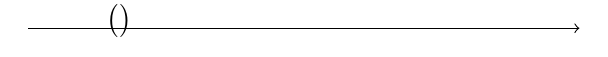
\begin{tikzpicture}
				\draw[->](-1,0)->(6,0);
				\IntervalLR{-1}{0}
				\def\skipInterval{0.5cm}%Khoảng cách đặt nhãn
				\IntervalGRF{}{}{\big(}{0}%Gạch xọc phải qua trái
				\IntervalLR{4}{6}%Gạch xọc trái qua phải
				\def\skipInterval{0.5cm}%Khoảng cách đặt nhãn
				\IntervalGRF{\big)}{4}{}{}%Gạch xọc phải qua trái
			\end{tikzpicture}
		\end{center}
		Vậy $A\cap B=[3;4)$ , $A\cup B=(0;+\infty)$.
	}
\end{ex}
%%%=============================%%%

%%%=============EX_5=============%%%
\begin{ex}%[0D1H3-4]
	[\textit{NH23-24-THPT Lê Trọng Tấn- Hồ Chí Minh}]
	Cho các tập hợp 
	\begin{eqnarray*}
		A=\{x \in \mathbb{R} \mid x \leq 4\}, B=[2 ; 5).
	\end{eqnarray*}
	Xác định $A \cup B$, $A \cap B$, $A \setminus B$, $\mathrm{C}_{\mathbb{R}} A$.
	\loigiai{
		Ta có $A=(-\infty;4]$, do đó  
		\begin{multicols}{4}
			\begin{itemize}
			\item $A\cap B =[2;4]$.
			\item $A\cup B =(-\infty;5)$.
			\item $A\setminus B=(-\infty;2)$.
			\item $\mathrm{C}_{\mathbb{R}}A =(4;+\infty)$.
		\end{itemize}
		\end{multicols}		
	}
\end{ex}
%%%=============================%%%

%%%=============EX_6=============%%%
\begin{ex}%[0D1H3-4]
	[\textit{GHKI NH23-24-THPT Chu Văn An - Quảng Ngãi}]
	Cho $A=\{x \in \mathbb{R}, x \leq 4\}$ và $B=\{x \in \mathbb{R}, 0\leq x < 5\}$.
	\begin{enumerate}
		\item  Viết tập $A, B$ dưới dạng khoảng, nửa khoảng, đoạn.
		\item  Tìm các tập $A\cap B, A\cup B, A\setminus B$
	\end{enumerate}
	\loigiai{
		\begin{enumerate}
			\item Ta có $A = (-\infty; 4]$ và $B = [0;5)$.
			\item Ta có $A \cap B = [0;4]$; $A \cup B = (-\infty; 5)$ và $A\setminus B = (-\infty; 0)$.
		\end{enumerate}
	}
\end{ex}
%%%=============================%%%

%%%=============EX_7=============%%%
\begin{ex}%[0D1H3-4]
	[\textit{GHKI NH23-24-THPT Chuyên Lê Hồng Phong-Quảng Nam}]
	Cho tập hợp $A=(-10; 5)$ và tập hợp $B=[0;+\infty)$. Xác định các tập hợp $A \cap B$; $A \cup B$; $B \setminus A$; $\mathrm{A} \cap \mathbb{N}$.
	\loigiai{
		Biểu diễn tập hợp $A=(-10; 5)$ và tập hợp $B=[0;+\infty)$ trên trục số ta được
		\begin{center}
			\begin{tikzpicture}[scale=1,>=stealth, font=\footnotesize,line join=round,line cap=round]
				\def\xmin{-5}\def\xmax{5}
				\node at (\xmin-2.5,0)[right]{$A=(-10;5)$};
				\draw[->] (\xmin,0)--(\xmax,0);
				\node at (\xmin-2.5,-1)[right]{$B=[0;+\infty)$};
				\draw[->] (\xmin,-1)--(\xmax,-1);
				\path (-2,0)node[shift={(90:5mm)}]{$-10$}(-2,0)node{$\big($}
				(3,0)node[shift={(90:5mm)}]{$5$}(3,0)node{$\big)$};
				\fill[pattern=north west lines]
				(\xmin,-0.1) rectangle (-2,0.1)
				(\xmax-0.2,-0.1) rectangle (3,0.1);
				\path (0,-1)node[shift={(90:5mm)}]{$0$}(0,-1)node{$\big[$}
				(\xmax,-1)node[shift={(90:5mm)}]{$+\infty$}
				;
				\fill[pattern=north west lines]
				(\xmin,-1.1) rectangle (0,-0.9)
				;
			\end{tikzpicture}
		\end{center}
		Từ đó ta suy ra
		\begin{multicols}{4}
			\begin{itemize}
			\item $A \cap B=[0;5)$.
			\item $A \cup B=(-10;+\infty)$.
			\item $B \setminus A=[5;+\infty)$.
			\item $A \cap \mathbb{N}=\{0; 1; 2; 3; 4\}$.
		\end{itemize}
		\end{multicols}
	}
\end{ex}
%%%=============================%%%

%%%=============EX_8=============%%%
\begin{ex}%[0D1V3-3]
	[\textit{HKI NH23-24-THPT Chuyên Lê Khiết-Quảng Ngãi}]
	Cho hai tập hợp $A=\{x \in \mathbb{R},|x+2|\leq 1\}$ và $B=(m+1;+\infty)$. Tìm điều kiện của tham số $m$ để $A\cap B=\varnothing$.
	\loigiai{
		Ta có $|x+2|\leq 1 \Rightarrow -1\leq x+2\leq 1 \Leftrightarrow -3\leq x\leq -1$.\\
		Vậy  $A=[-3;-1]$. Để $A\cap B=\varnothing$ thì $m+1\geq -1\Leftrightarrow m\geq -2$.\\
		Do đó với $m\geq -2$ thì $A\cap B=\varnothing$.
	}
\end{ex}
%%%=============================%%%

%%%=============EX_9=============%%%
\begin{ex}%[0D1V3-4]
	[\textit{GHK1 lớp 10 NH23-24-THPT Thanh Miện 2-Hải Dương}]
	\begin{enumerate}
		\item[a)] Tìm hiệu $\left[ 1;8 \right) \setminus \left[ 2; 7 \right)$.
		\item[b)] Cho hai tập hợp $A=[2;7]; \,\, B=(m-1; m)$. Tìm giá trị của $m$ để $A \cap B = \varnothing$.
	\end{enumerate}
	\loigiai{
		\begin{enumerate}
			\item[a)] Ta có $\left[ 1;8 \right) \setminus \left[ 2; 7 \right) = \left[1;2 \right) \cup \left[7;8 \right)$.
			\item[b)] Ta có $C_{\mathbb{R}}A = \left( -\infty; 2 \right) \cup \left( 7; +\infty \right)$.\\
			$A \cap B = \varnothing \Leftrightarrow B \subset C_{\mathbb{R}}A \Leftrightarrow \hoac{& m \leq 2 \\ & m-1 \geq 7} \Leftrightarrow \hoac{& m \leq 2 \\ & m \ge 8.}$
		\end{enumerate}
	}
\end{ex}
%%%=============================%%%

%%%=============EX_10=============%%%
\begin{ex}%[0D1V3-4]%[Dự án đề kiểm tra Toán 10 GHKI NH23-24- Phạm Văn Long]%[THPT TRẦN VĂN QUAN  - BÀ RỊA - VŨNG TÀU]
	[\textit{GHKI NH23-24-THPT TRẦN VĂN QUAN  - BÀ RỊA - VŨNG TÀU}]
	\begin{enumerate}
		\item  Cho $A=(-\infty; 5)$, $B=(-2; 8]$. Tìm $A\cap B$ và $A\setminus B$.
		\item  Cho tập hợp $A=[m; m+2]$, $B=[-1; 2]$ với $m$ là tham số. Tìm $m$ để $A\subset B$.
	\end{enumerate}
	\loigiai{
		\begin{enumerate}
			\item  Ta có $A \cap B=(-2 ; 5), A \setminus B=(-\infty ;-2]$.
			\item  Để $A \subset B$ thì $-1 \leq m<m+2 \leq 2 \Leftrightarrow \heva{&m \geq - 1\\&m + 2 \leq 2}\Leftrightarrow \heva{&m \geq-1\\&m \leq 0} \Leftrightarrow -1 \leq m\leq 0$.\\
			Vậy $-1 \leq m\leq 0$ thì $A\subset B$.
		\end{enumerate}
	}
\end{ex}

%%%=============================%%%

